\documentclass{standalone}
\usepackage[dvipsnames,svgnames,x11names]{xcolor}
\usepackage{tikz}
\usepackage{pgfplots}
\pgfplotsset{compat = 1.12}
\usepackage{../thesismath}
\begin{document}
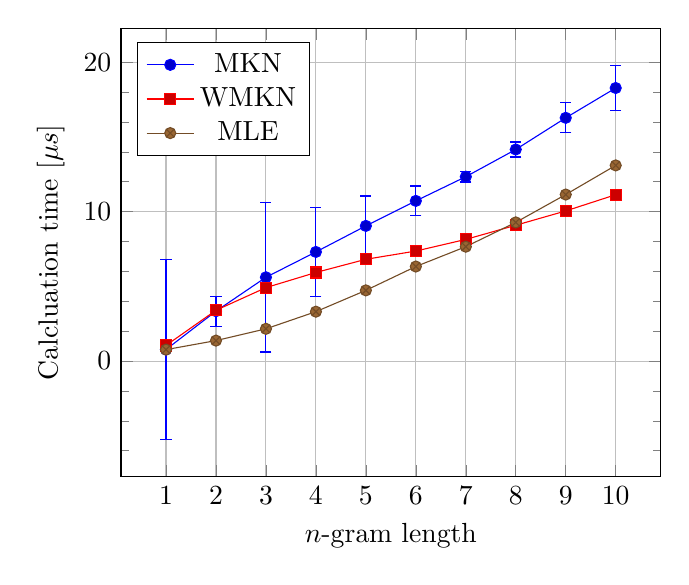
\begin{tikzpicture}[baseline]

\begin{axis}[
  xlabel = {$n$-gram length},
  xtick = {1, ..., 10},
  ylabel = {Calcluation time [${\mu}s$]},
  minor y tick num = 4,
  grid = major,
  legend entries = {{MKN}, {WMKN}, {MLE}},
  legend pos = north west,
]

% MKN
\addplot+[
  error bars/.cd,
  y dir = both,
  y explicit,
] table[y error = us_error] {
  n   us      us_error
  % sampled at N = 1000
  1   0.773   6
  2   3.339   1
  3   5.607   5
  4   7.303   3
  5   9.045   2
  6   10.719  1
  7   12.337  0.35
  8   14.159  0.5
  9   16.277  1
  10  18.274  1.5
};

% WMKN
\addplot table {
  n   us
  % sampled at N = 1000
  1   1.045
  2   3.398
  3   4.914
  4   5.928
  5   6.811
  6   7.362
  7   8.142
  8   9.089
  9   10.047
  10  11.133
};

% MLE
\addplot table {
  n   us
  % sampled at N = 1000
  1   0.766
  2   1.370
  3   2.157
  4   3.306
  5   4.731
  6   6.327
  7   7.654
  8   9.281
  9   11.144
  10  13.094
};

\end{axis}

\end{tikzpicture}
\end{document}
